\documentclass{article}

\documentclass[11pt]{article}
\usepackage{amssymb, amsmath}
\usepackage{algpseudocode}
\usepackage{algorithm}
\usepackage{array}
\usepackage{graphicx}
\usepackage{caption}
\usepackage{subcaption}
\usepackage{mathtools}
\usepackage{stmaryrd}
\usepackage{trimclip}
\usepackage[margin = 1.3in]{geometry}
\usepackage{mathrsfs}
\usepackage[T1]{fontenc}
\usepackage[utf8]{inputenc}
\usepackage{lmodern}
\usepackage{graphicx}
\usepackage[skip=2pt, font=scriptsize]{caption}
\usepackage[english]{babel}
\usepackage{csquotes}
\usepackage[notes,backend=biber]{biblatex-chicago}
\usepackage{ccpaper}

\bibliography{references}
\setlength\parindent{0pt}
\setlength\parskip{5pt}
%\captionsetup[figure]{font=small,labelfont=small}



\newlength{\nnearrowheight}
\newlength{\ssearrowheight}
\settoheight{\nnearrowheight}{$\nnearrow$}
\settoheight{\ssearrowheight}{$\ssearrow$}
\newcommand{\bQ}{\mathbb{Q}}
\newcommand{\bR}{\mathbb{R}}
\newcommand{\bC}{\mathbb{C}}
\newcommand{\bN}{\mathbb{N}}
\newcommand{\bZ}{\mathbb{Z}}
\newcommand{\bottomofnnearrow}{\makebox{\clipbox{0pt 0pt 0pt {.5\totalheight}}{$\nnearrow$}}}
\newcommand{\topofnnearrow}{\raisebox{.37\nnearrowheight}[.5\nnearrowheight][0pt]{\makebox{\clipbox{0pt {.5\totalheight} 0pt 0pt}{$\nnearrow$}}}}
\newcommand{\bottomofssearrow}{\makebox{\clipbox{0pt 0pt 0pt {.5\totalheight}}{$\ssearrow$}}}
\newcommand{\topofssearrow}{\raisebox{.37\ssearrowheight}[.5\ssearrowheight][0pt]{\makebox{\clipbox{0pt {.5\totalheight} 0pt 0pt}{$\ssearrow$}}}}
\newcommand{\upweakto}{\mathrel{%
    %\bottomofnnearrow%
    \hspace*{-.3pt}\makebox[0pt]{$-$}\hspace*{.35pt}%
    \topofnnearrow\hspace*{-.65pt}%
}}
\newcommand{\downweakto}{\mathrel{%
    %\hspace*{-.65pt}\topofssearrow%
    \hspace*{-.7pt}\makebox[0pt]{$-$}\hspace*{.35pt}%
    \bottomofssearrow%
}}

\DeclarePairedDelimiter\abs{\lvert}{\rvert}%
\DeclarePairedDelimiter\norm{\lVert}{\rVert}%

\makeatletter
\let\oldabs\abs
\def\abs{\@ifstar{\oldabs}{\oldabs*}}
%
\let\oldnorm\norm
\def\norm{\@ifstar{\oldnorm}{\oldnorm*}}
\makeatother
\DeclareMathOperator{\ord}{ord}
\DeclareMathOperator{\sech}{sech}

\newcolumntype{L}{>{$}l<{$}}
\newcommand\cpair[2]{%
\begin{tabular}{LL}#1 & #2\end{tabular}}
\algrenewcommand{\algorithmiccomment}[1]{\hfill#1}

\title{Taylor Series and The Cauchy Integral Formula for Matrix Functions \\ \small{A Comparative Analysis}}

\author{Farid Kaveh}

\begin{document}
\maketitle
\section{Abstract \& Motivation}
Matrix functions of the form $f(A)$ where $f$ is a scalar function $D \subseteq \bC \rightarrow \bC$ are used in a variety of areas, including numerical solutions to PDEs, Markov models, control theory, theoretical particle physics, computer graphics, and others. These scalar functions of matricies are defined via the Jordan Normal Form (JNF), Taylor series, and Cauchy integral definitions. These definitions are equivalent where they are valid. However, there are different sufficient conditions for the validity of each definition. Morever, when used to numerically calculate $f(A)$, these definitions exhibit different convergence and stability behaviours.

The Cauchy integral definition may exhibit several advantages over the others in computational settings, including in flexibility and numerical stability. However, here we are interested in comparing its algorithmic complexity and convergene behaviour to that of the Taylor series method in the case where $f$ is entire. To this end we analyse the complexity of the Cauchy and Taylor algorithms beginning from the basic routines for inversion and exponentiation that are used. We investigate the complexity of a number of algorithms intended for matrix inversion and polynomial evaluation. We then apply these algorithms to calculate $f(A)$ using the Cauchy integral and Taylor series definitions. We analyze the algorithmic complexity of each method and compare the speed and stability of our implementation using some examples.



\section{Background Theory}

Throughout this text we will refer to the trapezium rule approximation to the Cauchy integral definitions for $f(A)$ (see section 2.3) as the 'Cauchy algorithm' or 'Cauchy method' and likewise for the truncated Taylor series approximation to $f(A)$ we will write the 'Taylor algorithm' or 'Taylor method'. We also assume that $A$ is a square matrix and we use $n$ to denote its size, and so if we say that a certain process is $\Theta(f(n))$, then the input size $n$ is the size of $A$.

In analysing the computational complexity of algorithms, we assume the Random Access Machine (RAM) model of computation. Roughly, this means that each line of code will be executed by the machine one after the other. We may then assign the appropriate number of constant time operations that are required to execute each line of code. Summing these across the entire algorithm will give its complexity. We will consider addition, subtraction, multiplication, division, assignment, and boolean evaluation to be constant time operations. There are no simulataneuous operations taking place at any point under the RAM model.

When we refer to matrix functions, we mean objects of the form $f(A) \in \bC^{n\times n}$ where $f$ is a function $\bC \rightarrow \bC$ extended to $\bC ^{n \times n}$ by one of the following definitions:

\subsection{Jordan Canonical Form}
If $f$ is defined on the spectrum of $A$, i.e. the values
$$ f^{(j)}(\lambda_i), \; \; j = 0:n_i-1, \; \; i = 1:k$$
exist for $n_i$ the order of the largest Jordan block in which $\lambda_i$ appears. Then
\begin{equation}
  f(A) \coloneqq \Lambda f(J) \Lambda^{-1}
\end{equation}

where $J$ is the JCF of $A$ and for each Jordan block $J_i$

$$f(J_i) \coloneqq \begin{bmatrix} f(\lambda_i) && f'(\lambda_i)
&& \ldots && \frac{f^{(n_i-1)}(\lambda_i)}{(n_i -1)!} \\
&& f(\lambda_i) && \ddots && \vdots \\
&& && \ddots && f'(\lambda_i) \\
&& && && f(\lambda_i) \end{bmatrix}$$

\subsection{Taylor's expansion}
If $f$ has a taylor expansion about $z_0$ converging on a disc $D_R(z_0)$ such that we have for some matrix norm $||\cdot||$, $|| A - z_0I|| < R $.  Then

\begin{equation}
  f(A) \coloneqq \sum_{n=0}^{\infty} f_n(A - z_0I)^n
\end{equation}

\subsection{Cauchy Integral formula}

If $f$ is analytic on a domain $D$ and $\gamma$ is  a simple, closed, positvely aligned contour in $D$ such that $\sigma(A)$ lies inside of $\gamma$, then we may define

\begin{equation}
  f(A) \coloneqq \frac{1}{2\pi i}\int_{\gamma} f(\zeta)(A - \zeta I)^{-1}
\end{equation}

We included the JNF form definition for completeness, but in this project we will only be interested in the latter two representation of $f(A)$ presented above. Note that given any two of these definitions are valid for a given $(f,A)$, then they are equivalent. However, it will not always be the case that every definition is valid for this pair.

To numerically compute $f(A)$ using the Taylor expansion definition, we may truncate the series and sum finitely many terms. To do this computation using the Cauchy integral definitions, we will use the periodic trapezium rule approximation to the integral. In general, the periodic trapezium rule approximation to an integral on the interval $[0,2\pi]$ is given by:

$$ \int_0^{2\pi} f(\theta) \: d\theta \approx Q_Nf \coloneqq \frac{2\pi}{N}\sum_{j=0}^{N-1}f(\theta_j), \; \; \theta_j = \frac{2\pi j}{N},$$

hence the Cauchy integral method can be approximated by

$$ \frac{1}{2\pi i} \int_\gamma f(\zeta)(A - \zeta I)^{-1}
\: d\zeta \approx \frac{1}{iN}\sum_{j=0}^{N-1} f\left(\gamma(\theta_j)\right)\gamma'(\theta_j)(\gamma(\theta_j)I - A)^{-1}.$$

Here $\gamma$ is parameterised by $\theta \in [0,2\pi)$. In other words, we may approximate $f(A)$ \textit{either} by a finite sum of powers of $A$ \textit{or} by a finite sum of inverses involving $A$.
\section{Fundamental agorithms: inversion and exponentiation}

\subsection{Inversion}
For a general $A \in \bC^{n \times n}$ inversion is computationally equivalent to computing the reduced-row-echelon form of the matrix. This can be done via Gaussian elimination which for a dense matrix is $\Theta(n^3)$. Below is a piece of pseudocode showing the steps of this algorithm, along with the computational cost of each step. Note that in the psuedocode we use $\gets$ to indicate assignment and preserve the equality sign for denoting boolean evaluation.


\begin{algorithm}
\caption{Row-echelon form by Gaussian elimination}
\begin{algorithmic}[1]
\Procedure{Gaussian reduction}{$A\in \bC^{n \times n}$}   \Comment \cpair{\text{number of steps}}{}
\For {$ 1 \leq k \leq n-1$}   \Comment \cpair{$ \scriptstyle n-1$}{}

    \If {$A[k, k] = 0$} \Comment \cpair{$ \scriptstyle \sum_{k=1}^{n-1}(n-k) $}{}
                \State row $\gets A[k, :]$ \Comment \cpair{$\scriptstyle n$}{}
                \State $A[k, :] \gets A[j, :]$ \Comment \cpair{$\scriptstyle n$}{}
                \State $A[j, :] \gets$ row \Comment \cpair{$\scriptstyle n$}{}
                \State \textbf{break}
                \EndIf
            \EndFor
        \EndIf
    \If {$A[k, k] = 0$}
        \State \textbf{continue}
    \EndIf

    \For {$ k+1 \leq i \leq n$} \Comment \cpair{\text{(for whole loop)}}{$\scriptstyle \sum_{k=1}^{n-1}(n-k)(n-k-1)$}
        \State multp $\gets -A[i,k]/A[k,k]$
        \State $A[i, k:\text{end}] \gets A[i, k:\text{end}] + \text{multp}\cdot A[k,k:\text{end}]$
        \EndFor
    \EndFor
    \EndProcedure
\end{algorithmic}
\end{algorithm}

Now adding up the number of steps, and using the change of variable $j = n-k$, we find:

\begin{align*}
    \text{number of steps} &= n-1 + \sum_{k=1}^{n-1}(n-k) + n + n + n + \sum_{k = 1}^{n-1}(n-k)(n-k-1) \\
    &= 4n - 1 + \sum_{j=1}^{n-1}j + \sum_{j=1}^{n-1}j(j-1) \\
    &= 4n -1 \frac{n(n-1)}{2} - \frac{n(n-1)}{2} +\frac{1}{6}n(n-1)(2n-1)\\ &= 4n -1 + \frac{1}{6}n(n-1)(2n-1) \in \Theta(n^3)
\end{align*}
If we consider Gaussian redution to row echelon form as reducing the matrix to a similar upper triangular matrix, then the process of going from row echelon form to reduced row echelon form will generally be computationally cheaper than the symmetric problem of reducing $A$ to a similar lower triangular matrix. Hence we have indeed that matrix inversion via Gaussian elimination is $\Theta(n^3)$.

The method of inversion through reduction to r.r.e form is completely general and does not assume anything about $A$ (aside from invertability). There are other general algorithms for inversion of matricies, but they also have a worst case complexity of $\Theta(n^3)$.

However, if we allow some assumptions on $A$, we may be able to simplify the task of inverting it. An interesting and potentially very useful example is the one where $A$ is a toeplitz matrix with non-zero principle minors. Recall that a toeplitz matrix is one with entries $ a_{ij} = a_{(i-j)}$ for all $i, \: j$, or in other words, a matrix of the form

$$ A = \begin{pmatrix} a_0 && a_{-1} && a_{-2} && \ldots && a_{-n} \\
a_{1} && a_0 && a_{-1} && \ddots && \vdots \\
a_{2} && a_{1} && \ddots && \ddots && a_{-2} \\
\vdots && \ddots  && \ddots && a_{0} && a_{-1} \\
a_{n} && \ldots && a_{2} && a_1 && a_0
\end{pmatrix}.$$

A principle minor of $A$ is the determinant of $A$ after the $k$-th row and column have been removed for $k \in I \subseteq \mathcal{P}\left(\{1, \ldots, n\} \right)$.

With these assumptions on $A$, there exists a $\Theta(n^2)$ algorithm for inversion due to Trench (1964) \autocite{Trench}. In fact while Trench stated the result for non-Hermitian matricies, he proved the correctness of the algorithm for $A$ toeplitz, Hermitian, and postive definite; however in the 1968 paper \textit{'Toeplitz Matrix Inversion: The Algorithm of W. F. Trench'} Shalhav Zohar proves the validity of the algorithm for a non-Hermitian matrix and relaxes the positive definite condition to that of non-singular principle minors. \autocite{Zohar} We begin with a brief outline of the algorithm as described by Zohar's (borrowing his notation), but for a detailed proof of it's validity or relationship to the toeplitz structure of $A$ see the original paper.

\textbf{The Trench Algorithm}
We denote the transpose of a column vector $b$ by $\tilde{b}$ and we write $\hat{b}_i = b_{n-i}$ where $n$ is the dimension of $b$. The problem is of inverting $L_{n+1}$ toeplitz

$$ L_{n+1} = \begin{pmatrix} 1 && \tilde{a} \\
 r && L_n \end{pmatrix},$$

 where $a, r$ are $n \times 1$ column vectors. Denoting $a_i = \rho_{-i}$, $r_i = \rho_i$, and $B_{n+1} = L_{n+1}^{-1}$, we may find $B_{n+1}$ as below:

 let

 $$\lambda_1 = 1-\rho_{-1}\rho_{1}, \; \; e_1= -\rho_{-1}, \; \; g_1 = -\rho_1$$

 and define recursively for $1 \leq i < n$ the quantities

 \begin{align*}
     \eta_i &= -(\rho_{-(i+1)} + \tilde{e}_i \hat{a}_i) \\
     \gamma_i &= -(\rho_{i+1} + \tilde{r}_i\hat{g}_i) \\
     e_{i+1} &= \begin{pmatrix} e_i + \frac{\eta_i}{\lambda_i}\hat{g}_i \\
     \frac{\eta_i}{\lambda_i}\end{pmatrix}; \; \; \hat{g}_{i+1} = \begin{pmatrix} \frac{\gamma_i}{\lambda_i} \\
     \hat{g}_i + \frac{\gamma_i}{\lambda_i}e_i  \end{pmatrix} \\
     \lambda_{i+1} &= \lambda_i - (\eta_i\gamma_i/\lambda_i),
 \end{align*}

 then we have for $B_{n+1}$

 \begin{align*}
     (B_{n+1})_{11} &= 1/\lambda_n \\
     (B_{n+1})_{1,j+1} &= \frac{(e_n)_j}{\lambda_n}\\
     (B_{n+1})_{i+1,1} &= \frac{(g_n)_i}{\lambda_n} \\
     (B_{n+1})_{i+1,j+1} &= (B_{n+1})_{ij} + \frac{1}{\lambda_n}(g\tilde{e} - \hat{e}\tilde{\hat{g}})_{ij},   \; \;   1 \leq i,j < n.
 \end{align*}

 In this method there are $n-1$ recursive steps to find $e_n, g_n$ and $\lambda_n$. The $i$-th step involves $ci$ constant time processes for constant $c$, hence the recurisve steps include $\sim \frac{cn^2}{2}$ constant time processes in total. To evaluate $B_{n+1}$ the main computational task is to construct  $g\tilde{e} - \hat{e}\tilde{\hat{g}}$ which is also of $n^2$ complexity. So the trench algorithm terminates in $\Theta(n^2)$ time.

 While the assumptions on $A$ required by the Trench algorithm seem quite strong, we often meet such matricies in applications to PDE's. For instance, consider the matrix representation of the Jocabi operator, $J$, in the Chebyshev basis can be represented by an infinite toeplitz matrix (in fact it is also tridiagonal). Now if some smooth function $g$ has a Chebyshev given by coefficient $u_i$, then given another function $\phi$, we may cheaply calculate the Chbyshev expansion of $\phi g$ by computing $\phi(J)$ using the Trench algorithm and the Trench method, and then writing

 $$ \tilde{u} = \phi(J)u, $$

 where $\tilde{u}$ will be the Chebyshev coefficients of $\phi g$.

 \textbf{Remark.} Note that for a general matrix which is defined by $n^2$ quantities, the algorithm we gave for inversion is $\Theta(n^3)$, and for a toplitz matrix which is defined by $2n-1$ quantities (the first row and column) we have a $\Theta(n^2)$ algorithm. We know also that there is a lower bound of $\Omega(n^2\log n)$ on the complexity of a general method for matrix inversion.\autocite{tveit2003complexity} This could hint at a more general result for the complexity of inverting a finite dimensional operator.


\subsection{Exponentiation}
Now we turn our attention to the problem of computing the $k-th$ power of a matrix when $k$ is large, which we will face when finding $f(A)$ through the Taylor series method. This may be done naively by multiplying $A$ by itself $k$ times, then the entire process will be $\Theta(kn^3)$, since matrix multiplication is $\Theta(n^3)$. If $k \approx n$ then this is $\Theta(n^4)$. If only require the $k-th$ power of $A$, then we may do better using the exponentiation by squaring method. Suppose we wish to compute $x^k$ for $x \in R$ ring. Then we may write $k = \sum c_m2^m$ with $c_m \in \{0,1\}$. In particular $n$ has the binary representation $c_Nc_{N-1}\ldots c_2c_1$ where $K = \lfloor \log_2(k) \rfloor$. Then if $r_m = x^{2^m}$, (which we may calculate in $m$ multiplications), we have that $x^k = \prod r_m^{c_m}$. Hence we have calculated $x^k$ in $\sim 2\log k$ multiplications. Below is an implementation of this algorithm in pseudocode.

However, in evaluating truncated Taylor series in $A$ we will need all powers $A^0, A, \ldots, A^{k-1}, A^k$. In such a case it is best to evaluate the required matrcies by repeatedly multiplying by $A$. To efficiently evaluate truncations of the Taylor series we may use Horner's method which for an $N$-th degree polynomial has a computational cost of $(N-1)$ matrix multiplications.\autocite{Higham} See Algorithm 3 for an outline.

\begin{algorithm}\caption{Exponentiation by Squaring}\label{exp_sqr}\begin{algorithmic}[1]\Procedure{Exp by Squaring}{$x,n$}
    \State bin $=$ \textbf{str\_binary}($n$) \Comment{Assign binary string of $n$ to 'bin'}
    \State bin $\gets$ \textbf{reverse}(bin)     \Comment{reverse the string so we iterate from the 1's place up}
    \State $x\_exp \gets 1$
    \State $x_m \gets x$
    \If {bin[1] = '1'}
        \State $x\_exp \gets x$
    \EndIf

    \For {$2 \leq \text{digit} \leq \textbf{length}(\text{bin})$}
        \State $x_m \gets x_m \cdot x_m$
        \If {bin[digit] $=$ '1'}
            \State $x\_exp \gets x\_exp\cdot x_m$
        \EndIf
    \EndFor
    \State \textbf{return} $x\_exp$
    \EndProcedure
\end{algorithmic}
\end{algorithm}

\begin{algorithm}\caption{Horner's Polynomial Evaluation}\label{exp_sqr}\begin{algorithmic}[1]\Procedure{Horner's Method}{$A, F$} \Comment{$F$ is a vector of coefficients}
    \State $S_0 \gets F[N]A +F[N-1]I$ \Comment{$F[i]$ is the coeffcient of $A^i$}
    \For{$1 \leq i \leq N-1$}
        \State $S_{i} \gets AS_{i-1}+F[N-i-1]I$
    \EndFor
    \State \textbf{return} $S_{N-1}$
    \EndProcedure
\end{algorithmic}
\end{algorithm}

\section{Convergence \& Truncation Error}

We must consider two sources of error when deciding between the Cauchy and Taylor methods. The truncation error, and the floating point calculation rounding error. Here we will only be treating the truncation error.

Let us assume for a moment that approximations of the Taylor and Cauchy definitions of $f(A)$ converge at the same rate. In this case we may expect that in general comparable precision can be achieved in similar time since both methods involve computing $N$ matrix multipication/inversions and then summing up the resulting $N$ terms. This may differ in the case where $A$ is toeplitz with non-singular principle minors as discussed in 3.1.

One may then ask whether these methods do in fact converge at similar rates to $f(A)$. We know that for a periodic function, (such as $f$ on a simple closed contour $\gamma$) the trapezium rule approximation to the Cauchy integral formula converges exponentially to the true value of the integral, but this will not necessarily carry over to the case where the argument of $f$ is a matrix. We will now prove some results regarding Taylor series which will allow us to explore the convergence behaviour of the Taylor algorithm.

\begin{theorem}[Uniform convergence of Taylor series]
     Let $\sum_{k = 0}^\infty f_k(z-z_0)^k$ be the Taylor expansion of the function $f$ about the point $z_0$. Then if this expansion converges on and inside a circular contour $\gamma$ of radius $\rho$ about $z_0$, it converges uniformly to $f$ on the interior, and moreover the partial sums $\sum_{k = 0}^N f_k(z-z_0)^k$ converge to $f$ at least exponentially.
\end{theorem}

\textbf{Proof.}

Let $\gamma_C$ be a circular contour of radius $C\rho$ where $0 \leq C < 1$. Then $\abs{z - z_0} \leq C\rho$ for all $z$ in the interior of $\gamma_C$. We also have

\begin{align*}
    \abs{f_k} &= \abs{\frac{1}{2\pi i}\int_\gamma \frac{f(\zeta)\,d\zeta}{(\zeta -z_0)^{k+1}}} \\
    &\leq \frac{2\pi \rho}{2\pi} \frac{\sup_{\zeta\in \gamma}f(\zeta)}{\rho^{k+1}} = \frac{\sup_{\zeta\in \gamma}f(\zeta)}{\rho^k}
\end{align*}

If we then let $M = \sup_{\zeta \in \gamma}f(\gamma)$, we have the inequality
$$ f_k(z-z_0)^k \leq \frac{MC^k\rho^k}{\rho^k} = MC^k,$$

for all $k$. Then since the RHS is summable, we have by the Weistress M-test that $\sum_{k=0}^{\infty}f_k(z-z_0)^k$ converges uniformly on the interior of $\gamma$. To bound the error of the partial sums for a given $\gamma_C$ we have

\begin{align*}
    \abs{f(z) - \sum_{k=0}^N f_k(z-z_0)^k } &= \abs{\sum_{k = N+1}^\infty f_k(z-z_0)^k} \\
    &= M\sum_{k= N+1}^\infty C^k \\
    &= M\left(\frac{1}{1-C}-\frac{1-C^{N+1}}{1-C}\right) = \frac{MC^{N+1}}{1-C}.
\end{align*}
\hfill $\square$

While the above reassures us that the Taylor series behaves nicely, at least for $z \in \bC$, the convergence behaviour of matrix polynomials does not necessarily coincide with that of polynomials in $\bC$. Hence we state also the following theorem due to Mathias. \autocite{R.Mathias}

\begin{theorem}[Truncation error of the Taylor method]

If $f(z) = \sum_{k=0}^\infty f_kz^k$ has radius of convergence $\rho$, and $A \in \bC^{n\times n}$ with $\norm{A}_2 < \rho$, then the truncation error for $f(A)$ satisfies the follwing inequality

$$ \norm{f(A) - \sum_{k=0}^N f_kA^k}}_p \leq \frac{1}{(N+1)!}
\max_{t \in [0,1]} \norm{A^{N+1}f^{(N+1)}(tA)}_p,$$

where $\norm{\cdot}_p$ is any matrix norm.
\end{theorem}
\textbf{Proof.} See the Paper by Mathias R. $\square$

For many functions, bounding the quantity $\max_{t \in [0,1]} \norm{A^{N+1}f^{(N+1)}(tA)}_p$ is simple. For example, let $f(z) = e^z$ and $p=\infty$. Then $f^{(N+1)}(z) = f(z) = e^z$ and so

\begin{align*}
    \norm{A^{N+1}\exp(tA)}_\infty &= \norm{A^{N+1}\sum_{k=0}^\infty \frac{(tA)^k}{k!}}_\infty \\
    &\leq \sum_{k=0}^\infty\frac{\norm{t^kA^{N+1+k}}_\infty}{k!} \\
    &\leq \norm{A^{N+1}}_\infty \exp(\norm{A}_\infty).
\end{align*}

In the case where $\norm{A}_\infty < 1$ Theorem 4.2 clearly implies that the truncation error of the Taylor series method decreases super exponentially. In the lectures we found that for periodic $f$ the trapezium rule converges exponentially as the number of nodes increases. We are interested in the integral of $f$ on a closed simple contour, in which case the integrand will indeed be periodic. However, as we noted before, convergence results derived on the complex plane do not always apply to the case where the argument of $f$ is a matrix.

To establish the rate of convergence of $Q_Nf(A)$, figures (numbers) show the error of this approximation to the true value of $f(A)$ as measured by $\norm{\cdot}_\infty$ for some examples of $f$ entire. In producing these figures, we used matricies $A$ such that $\norm{A}_2 = 1$. This is in part to allow for ease of comparasion with the bound on the  Taylor series convergence we derived above. Taking the contour of integration to be of radius $r \approx 1$ also serves to avoid complicated stability and accuracy issues that may arise in trapezoidal approximations to the Cauchy integral formula as this radius gets large or small. \autocite[see]{Bornemann2011}

\begin{figure}
    \centering
    \begin{subfigure}[b]{0.3\linewidth}
        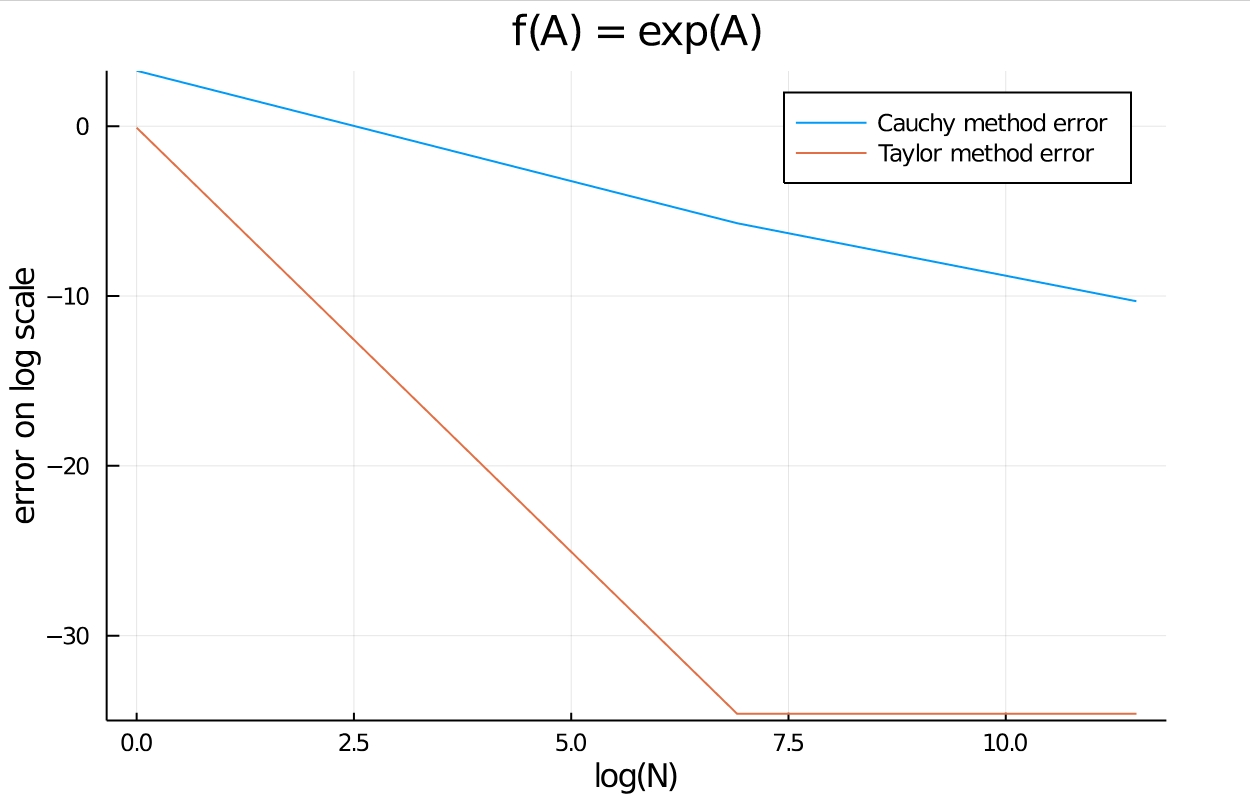
\includegraphics[width = \textwidth]{expA.jpg}
        \caption{}
        \label{}
    \end{subfigure}
    \begin{subfigure}[b]{0.3 \linewidth}
        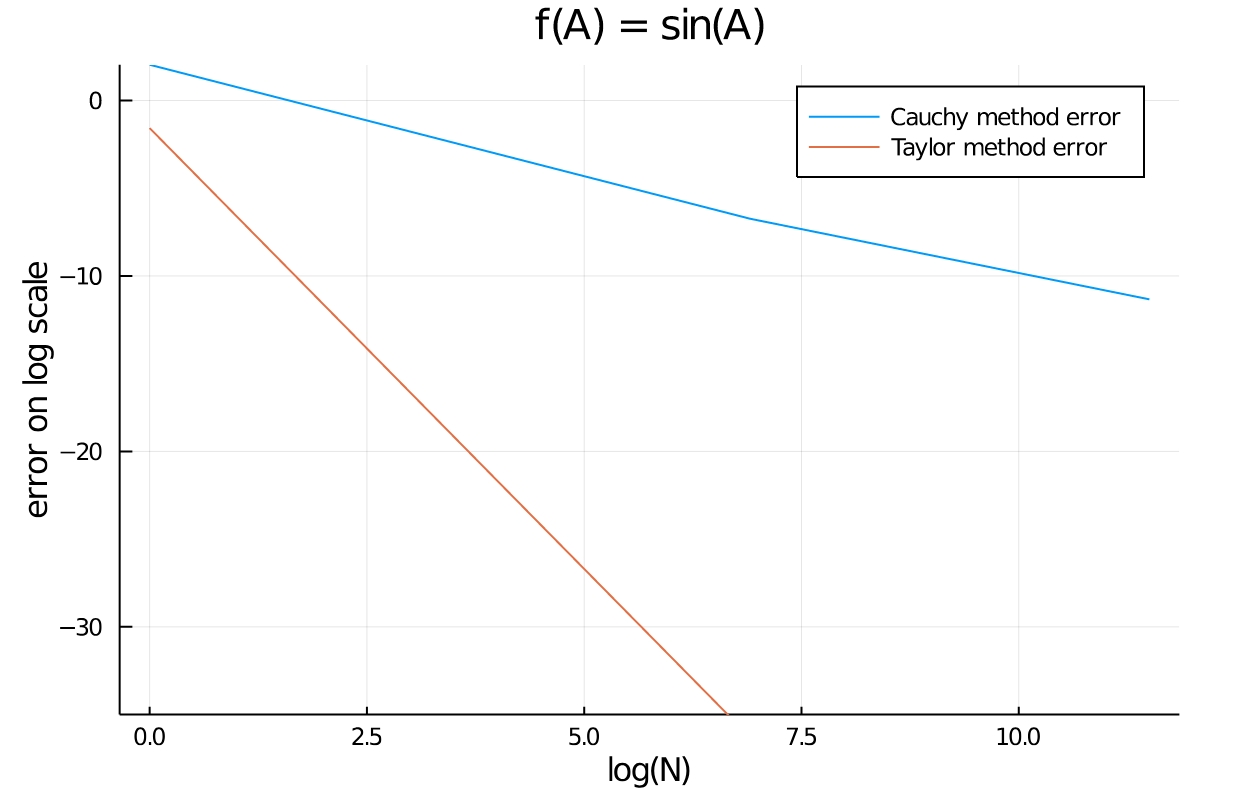
\includegraphics[width = \textwidth]
        {sinA.jpg}
        \caption{}
        \label{}
    \end{subfigure}
    \begin{subfigure}[b]{0.3 \linewidth}
        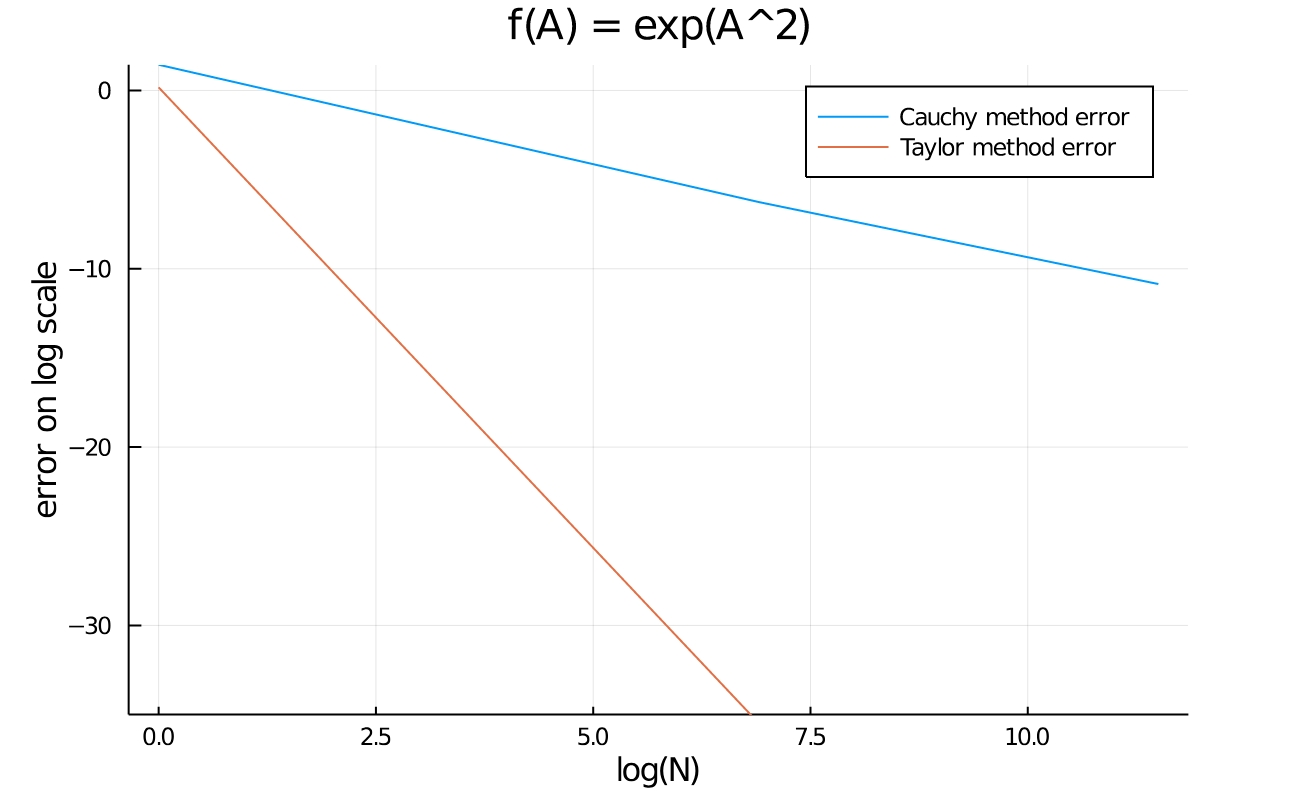
\includegraphics[width = \textwidth]
        {expA^2.jpg}
        \caption{}
        \label{}
    \end{subfigure}
    \caption[LoF entry]{Errors for the Cauchy and Taylor methods after $N$ summations and as measured by the $\norm{\cdot}_\infty$ norm. $A$ is a $5\times 5$ matrix. Note the log-log scale.}
    \label{fig:5by5}
\end{figure}

\begin{figure}
    \centering
    \begin{subfigure}[b]{0.3\linewidth}
        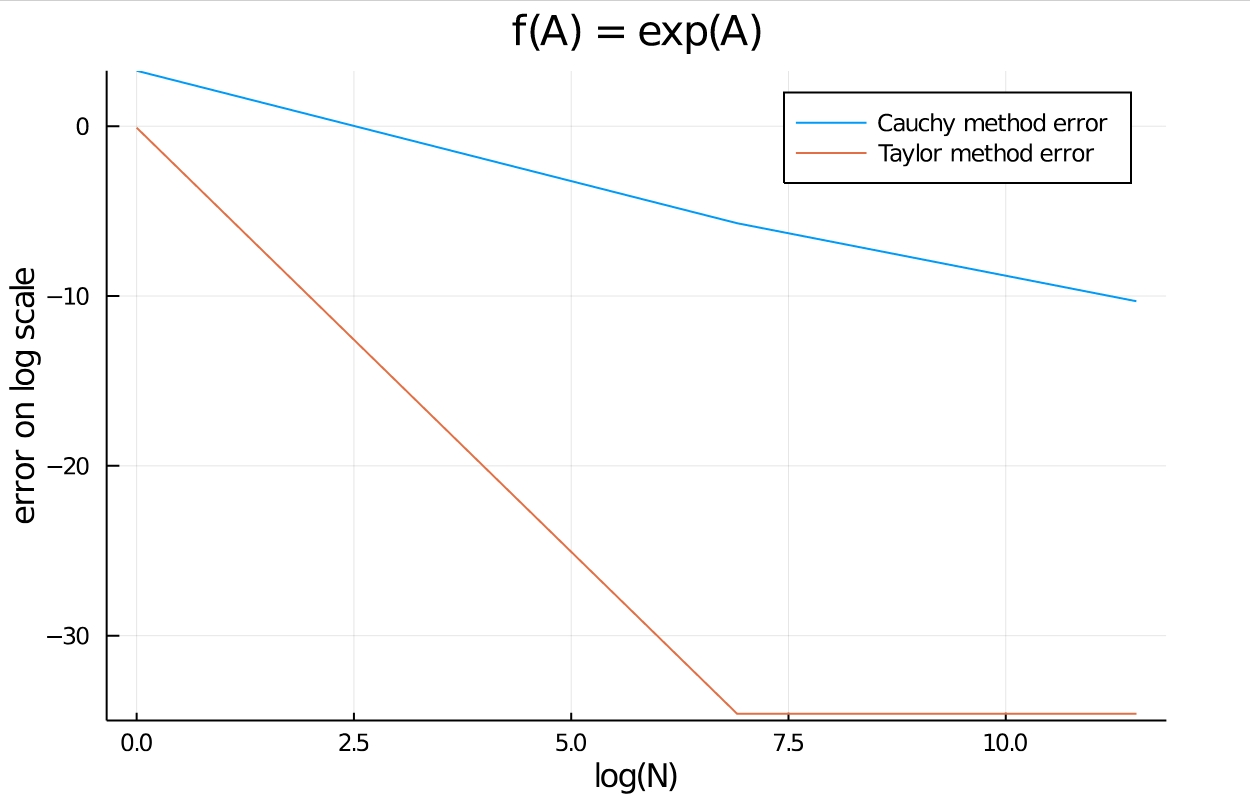
\includegraphics[width = \textwidth]{expA.jpg}
        \caption{}
        \label{}
    \end{subfigure}
    \begin{subfigure}[b]{0.3 \linewidth}
        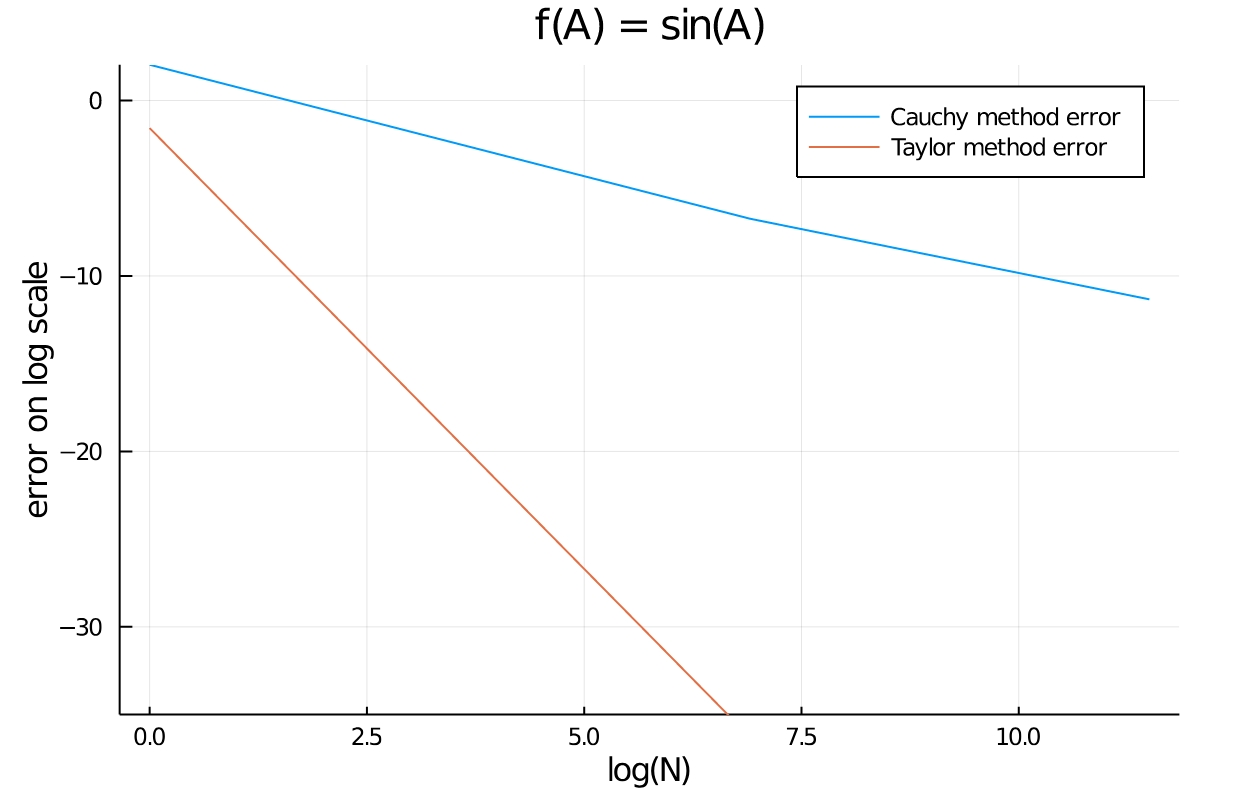
\includegraphics[width = \textwidth]
        {sinA.jpg}
        \caption{}
        \label{}
    \end{subfigure}
    \begin{subfigure}[b]{0.3 \linewidth}
        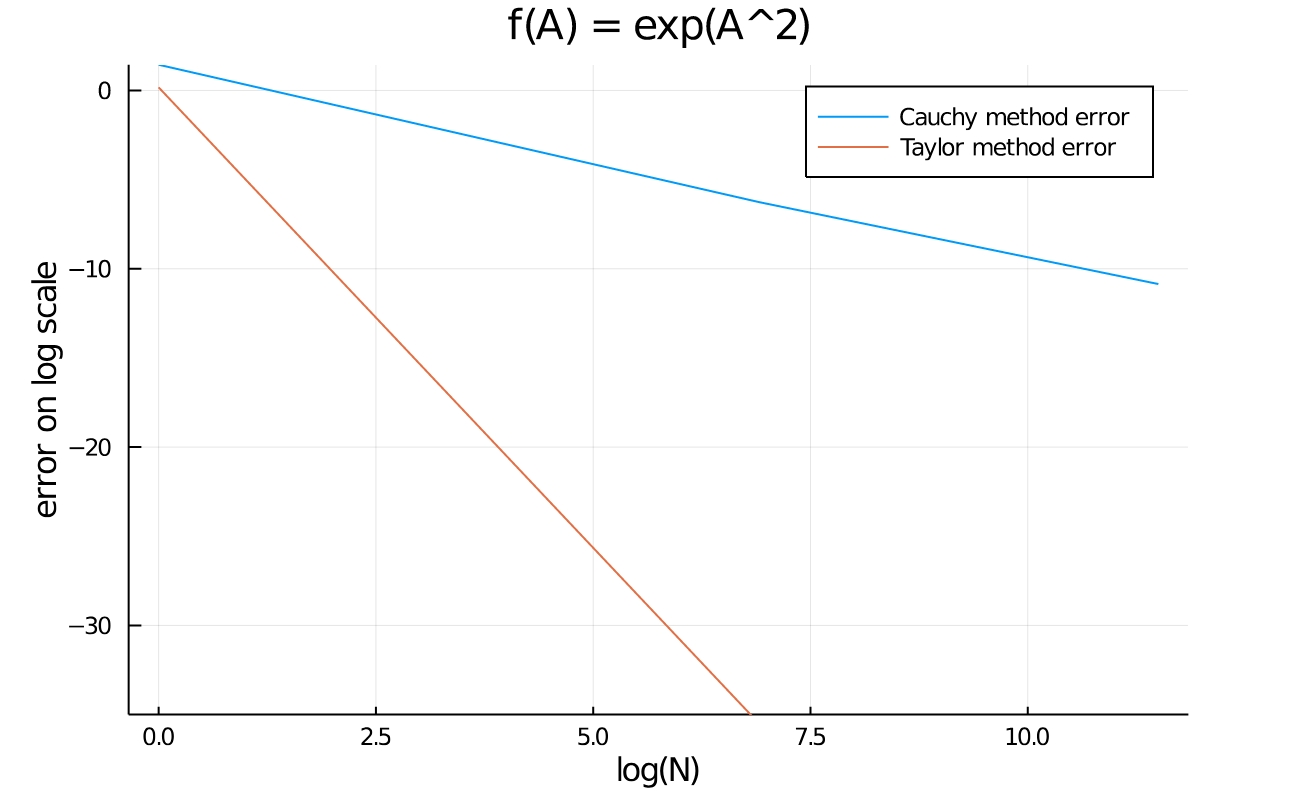
\includegraphics[width = \textwidth]
        {expA^2.jpg}
        \caption{}
        \label{}
    \end{subfigure}
    \caption[LoF entry]{These plots give the same information as in Figure ~\ref{fig:5by5} but here $A$ is $10 \times 10$}
    \label{fig:10by10}
\end{figure}



Most notably, what these figures show is that in practice floating point errors cannot be ignored, since neither method produces exponential or superexponential convergence. Both seem to be converging to the true value of $f(A)$ algebraically, however the curve for the Taylor method is very steep and indeed we reach machine precision with this method once $N \approx e^7$. These plots suggest that the Taylor method should be favored when we can only place weak assumptions on $A$, but $f$ is well behaved. We say that $f$ must be well behaved because if it has a branch cut it may not be possible to produce a Taylor series of $f$ with a disc of convergence that encapsulates the spectrum of $A$.

What is more promising is the consistency of the convergence behaviour across the different instances of the arguments $f$ and $A$.
\section*{Conclusions}
We showed that the fundamental processes in computing each term of the summation in the Taylor and Cauchy methods are of the same complexity, if we cannot place any assumptions on $A$. Furthermore we found that in our implementation of the algorithms, the Taylor method converges to the true value of $f(A)$ far more quickly. Albeit, both algorithms converge algebraically, which is slower than expected. This may have been due to our neglect of floating point rounding errors.

These results suggest that the Taylor method is more efficient when assumptions on $A$ are weak but those on $f$ are strong in the sense it does not have branch cuts. An analysis of the effect of the Trench algorithm on the time efficiency of the Cauchy method in the case of toeplitz $A$ remains to be had. It is also important to analyse the convergence of each algorithm with $f$ a rational function, which we have not done here.

\printbibliography

\end{document}
